% choose language here
\documentclass[a4paper,twoside,12pt,english]{ctuThesis2}
\usepackage[english]{babel}

\author{Student Hardworking}
\supervisor{Supervisor Strict}{A very famous institution}

% Consultant and second consultant. Comment out to ommit.
\consultant{Consultant Consulting}{An even more famous group}
\secondConsultant{Consultant Second}{Not that famous group}

% Comment out `titleEN` if your language is english
\title{O zvířatech}
% \titleEN{About animals}

\university{Forest university}
\faculty{School of Deer}
\department{Department of domestication}

% CZ/SK: Použijte 6. pád
\city{Praha}
\year{2022}

% your study major 
\major{Domestication}

% choose one of `BP`, `VU` or `DP` or rename it by whatever you like
\type{\BP}

\scanOfAssignment{specimen1.pdf}{specimen2.pdf}

% use `keywordsEN` for english translation, comment out if not needed
\keywords{chov, krmení}
% \keywordsEN{husbandry, feeding}

% use `abstractEN` for english translation, comment out if not needed
\abstract{
Pellentesque congue aliquet nulla quis vestibulum. Aenean vitae porttitor nunc. Praesent imperdiet erat eget justo dictum tempus. Proin pulvinar metus eget arcu elementum blandit. Duis et lacus id tellus blandit eleifend. Vestibulum eleifend molestie scelerisque. Pellentesque convallis ex sed ipsum faucibus, in fermentum nunc dignissim. Nullam eu eros non enim mattis porttitor. Nunc maximus, elit placerat elementum faucibus, eros nisi rhoncus leo, a porttitor nisl ligula ac libero. Integer fermentum eget dolor id tempus.
  A decent abstract.
}
% \abstractEN{Translation of the abstract}

% use e.g. 
% Prohlašuji, že jsem svou bakalářskou práci vypracoval samostatně a použil jsem pouze podklady (literaturu, projekty, SW atd.) uvedené v přiloženém seznamu.
% I hereby admit that this work is original and all used resources have been cited in bibliography. 
\proclamation{Some proclamation of originality}

% use e.g.
% Autor děkuje vedoucímu práce za cenné rady.
% The author is grateful to the supervisor for valuable  
\acknowledgement{
  Some acknowledgement
}

% style of page layout
\pagestyle{fancy}
\fancyfoot{}
\fancyhead[RO,LE]{\thepage}
\fancyhead[RE]{\nouppercase{\leftmark}}
\fancyhead[LO]{\nouppercase{\rightmark}}

\begin{document}

% frontmatter changes page numbers to roman etc
\frontmatter

\maketitle

\includeAssignment

\makeProclamation

\makeAcknowledgement

\makeAbstract

\makeTOC

% the text itself begins here
\chapter*{\AcronymsWord}
\addcontentsline{toc}{chapter}{\AcronymsWord}
\markboth{\AcronymsWord}{\AcronymsWord}
\begin{acronym}[TDMA]
    \acro{ann}[ANN]{Neuronová síť (\ti{Artificial Neural Network})}
    \acro{az}[AZ]{Aktivní zóna}
\end{acronym}


\listoffigures

% normal numbering by arabic numbers
\mainmatter

\stdindent
\stdskip

\chapter*{Úvod} % SEM NESAHEJTE!
\addcontentsline{toc}{chapter}{Úvod} % SEM NESAHEJTE!
\markboth{Úvod}{Úvod}
% \uv{Lorem ipsum} dolor sit amet, consectetur adipiscing elit. Suspendisse velit tellus, ornare at nisl vitae, mollis dignissim erat. Nulla facilisi. Nunc aliquet feugiat eros eu convallis. Donec iaculis lectus ac neque euismod ullamcorper. Cras iaculis malesuada enim ac hendrerit. Aenean porta, augue a ultricies vestibulum, tellus tellus mattis ante, sit amet efficitur tellus velit a enim. Phasellus tristique, ipsum sit amet placerat ullamcorper, turpis turpis fringilla ligula, ut mattis magna nibh id lorem. Morbi congue augue in arcu lobortis viverra. In lectus nisl, dignissim quis egestas quis, pulvinar sed odio. Mauris condimentum nisl suscipit, rutrum nibh vel, suscipit odio.

Pellentesque congue aliquet nulla quis vestibulum. Aenean vitae porttitor nunc. Praesent imperdiet erat eget justo dictum tempus. Proin pulvinar metus eget arcu elementum blandit. Duis et lacus id tellus blandit eleifend. Vestibulum eleifend molestie scelerisque. Pellentesque convallis ex sed ipsum faucibus, in fermentum nunc dignissim. Nullam eu eros non enim mattis porttitor. Nunc maximus, elit placerat elementum faucibus, eros nisi rhoncus leo, a porttitor nisl ligula ac libero. Integer fermentum eget dolor id tempus.

Something with itallic index $F_p$. And something with non-itallic $F\_p$. Sed purus enim, blandit sed interdum ut, fermentum at erat. Sed in elementum erat. In at enim nisl. Integer eu nibh sit amet quam ornare faucibus aliquam quis sem. Nunc vel nisl eu nunc congue viverra ac sagittis justo. Integer pharetra diam purus. Pellentesque dignissim est vel rutrum laoreet. Praesent id eros suscipit, porttitor nisi id, dignissim neque. Phasellus commodo volutpat nulla eget suscipit. Curabitur sit amet dapibus nisi. Donec consectetur nisl vitae neque vestibulum finibus. Duis sodales tempor ante, eu ultricies dolor bibendum ut.

Quisque id dignissim leo. Suspendisse tincidunt lacinia varius. Nunc a sem tristique, porta augue quis, tempor turpis. Pellentesque habitant morbi tristique senectus et netus et malesuada fames ac turpis egestas. Proin nulla sapien, pellentesque vitae magna sed, feugiat auctor dui. Duis nec porttitor velit. Suspendisse auctor malesuada mauris, at mattis est egestas et. Aliquam placerat molestie rutrum. Nunc tempus, est a ultricies luctus, dui leo hendrerit neque, quis dictum purus lacus et purus. Morbi aliquet elit et sodales pharetra. Morbi imperdiet viverra sagittis. Phasellus quam velit, pretium vel efficitur et, tempus ac metus. Donec non dapibus nibh. Vestibulum viverra cursus nisi. Phasellus vitae ipsum pretium, tempus mauris sagittis, tempus mi.

Maecenas dapibus erat non odio tristique porta. Suspendisse elementum nibh a nisl fermentum, eu blandit risus venenatis. Integer sed mi cursus, vestibulum dui in, gravida magna. Phasellus dictum maximus ultricies. Vivamus congue molestie ipsum, nec lobortis quam condimentum sit amet. In hac habitasse platea dictumst. Proin facilisis eleifend purus, ac egestas diam fermentum non. Aenean malesuada elit quis ligula faucibus porttitor. Etiam ornare ullamcorper orci, eget sagittis nulla fringilla ac. Ut ac metus ultricies, porttitor orci ac, accumsan erat. Nam eu elit elit. Integer vitae mi at leo elementum cursus ullamcorper eu lorem. aaaaaaaaaaaaaaa

\mdef{Parsevalova nerovnost}{parseval}{to je
Maecenas dapibus erat non odio tristique porta. Suspendisse elementum nibh a
nisl fermentum, eu blandit risus venenatis. Integer sed mi cursus, vestibulum
dui in, gravida magna. Phasellus dictum maximus ultricies. Vivamus congue
molestie ipsum, nec lobortis quam condimentum sit amet. In hac habitasse platea
dictumst. Proin facilisis eleifend purus, ac egestas diam fermentum non. Aenean
malesuada elit quis ligula faucibus porttitor. Etiam ornare ullamcorper orci,
eget sagittis nulla fringilla ac. Ut ac metus ultricies, porttitor orci ac,
accumsan erat. Nam eu elit elit. Integer vitae mi at leo elementum cursus
ullamcorper eu lorem. aaaaaaaaaaaaaaa
}

je v definici \ref{mdef:parseval}.

\mtheor{Velká Belkova}{belko}{aaaaaaaaaaaaaaaaa}

Belk citát je v~\ref{mtheor:belko}.

\mlemma{Malá Rzehulkova}{rzehulka}{PIVOOO!!!}


RRR citát je v~\ref{mlemma:rzehulka}.
\mcomm{Koment Mončin}{monca}{vám?
Quisque id dignissim leo. Suspendisse tincidunt lacinia varius. Nunc a sem tristique, porta augue quis, tempor turpis. Pellentesque habitant morbi tristique senectus et netus et malesuada fames ac turpis egestas. Proin nulla sapien, pellentesque vitae magna sed, feugiat auctor dui. Duis nec porttitor velit. Suspendisse auctor malesuada mauris, at mattis est egestas et. Aliquam placerat molestie rutrum. Nunc tempus, est a ultricies luctus, dui leo hendrerit neque, quis dictum purus lacus et purus. Morbi aliquet elit et sodales pharetra. Morbi imperdiet viverra sagittis. Phasellus quam velit, pretium vel efficitur et, tempus ac metus. Donec non dapibus nibh. Vestibulum viverra cursus nisi. Phasellus vitae ipsum pretium, tempus mauris sagittis, tempus mi.

}

Monča řekla komentář~\ref{mcomm:monca}
Quisque id dignissim leo. Suspendisse tincidunt lacinia varius. Nunc a sem tristique, porta augue quis, tempor turpis. Pellentesque habitant morbi tristique senectus et netus et malesuada fames ac turpis egestas. Proin nulla sapien, pellentesque vitae magna sed, feugiat auctor dui. Duis nec porttitor velit. Suspendisse auctor malesuada mauris, at mattis est egestas et. Aliquam placerat molestie rutrum. Nunc tempus, est a ultricies luctus, dui leo hendrerit neque, quis dictum purus lacus et purus. Morbi aliquet elit et sodales pharetra. Morbi imperdiet viverra sagittis. Phasellus quam velit, pretium vel efficitur et, tempus ac metus. Donec non dapibus nibh. Vestibulum viverra cursus nisi. Phasellus vitae ipsum pretium, tempus mauris sagittis, tempus mi.


\mex{jirka}{Jak si to máme představit?}

Jirka rekl~\ref{mex:jirka},
Quisque id dignissim leo. Suspendisse tincidunt lacinia varius. Nunc a sem tristique, porta augue quis, tempor turpis. Pellentesque habitant morbi tristique senectus et netus et malesuada fames ac turpis egestas. Proin nulla sapien, pellentesque vitae magna sed, feugiat auctor dui. Duis nec porttitor velit. Suspendisse auctor malesuada mauris, at mattis est egestas et. Aliquam placerat molestie rutrum. Nunc tempus, est a ultricies luctus, dui leo hendrerit neque, quis dictum purus lacus et purus. Morbi aliquet elit et sodales pharetra. Morbi imperdiet viverra sagittis. Phasellus quam velit, pretium vel efficitur et, tempus ac metus. Donec non dapibus nibh. Vestibulum viverra cursus nisi. Phasellus vitae ipsum pretium, tempus mauris sagittis, tempus mi.
Quisque id dignissim leo. Suspendisse tincidunt lacinia varius. Nunc a sem tristique, porta augue quis, tempor turpis. Pellentesque habitant morbi tristique senectus et netus et malesuada fames ac turpis egestas. Proin nulla sapien, pellentesque vitae magna sed, feugiat auctor dui. Duis nec porttitor velit. Suspendisse auctor malesuada mauris, at mattis est egestas et. Aliquam placerat molestie rutrum. Nunc tempus, est a ultricies luctus, dui leo hendrerit neque, quis dictum purus lacus et purus. Morbi aliquet elit et sodales pharetra. Morbi imperdiet viverra sagittis. Phasellus quam velit, pretium vel efficitur et, tempus ac metus. Donec non dapibus nibh. Vestibulum viverra cursus nisi. Phasellus vitae ipsum pretium, tempus mauris sagittis, tempus mi.
Quisque id dignissim leo. Suspendisse tincidunt lacinia varius. Nunc a sem tristique, porta augue quis, tempor turpis. Pellentesque habitant morbi tristique senectus et netus et malesuada fames ac turpis egestas. Proin nulla sapien, pellentesque vitae magna sed, feugiat auctor dui. Duis nec porttitor velit. Suspendisse auctor malesuada mauris, at mattis est egestas et. Aliquam placerat molestie rutrum. Nunc tempus, est a ultricies luctus, dui leo hendrerit neque, quis dictum purus lacus et purus. Morbi aliquet elit et sodales pharetra. Morbi imperdiet viverra sagittis. Phasellus quam velit, pretium vel efficitur et, tempus ac metus. Donec non dapibus nibh. Vestibulum viverra cursus nisi. Phasellus vitae ipsum pretium, tempus mauris sagittis, tempus mi.
Quisque id dignissim leo. Suspendisse tincidunt lacinia varius. Nunc a sem tristique, porta augue quis, tempor turpis. Pellentesque habitant morbi tristique senectus et netus et malesuada fames ac turpis egestas. Proin nulla sapien, pellentesque vitae magna sed, feugiat auctor dui. Duis nec porttitor velit. Suspendisse auctor malesuada mauris, at mattis est egestas et. Aliquam placerat molestie rutrum. Nunc tempus, est a ultricies luctus, dui leo hendrerit neque, quis dictum purus lacus et purus. Morbi aliquet elit et sodales pharetra. Morbi imperdiet viverra sagittis. Phasellus quam velit, pretium vel efficitur et, tempus ac metus. Donec non dapibus nibh. Vestibulum viverra cursus nisi. Phasellus vitae ipsum pretium, tempus mauris sagittis, tempus mi.

\chapter{Moje práce}
Tato práce třeba jednou bude hezká.

\section{Něco}
Aaargh.
\subsection{Menší něco}
Lalalalala. Chtěli bychom něco citovat. Tak třeba \cite{baker}.
\section{Ještě jedno něco}
Blalala. Kukni na obrazek~\ref{omnia.jpg}.


\pic{omnia.jpg}{Popis do seznamu obrazku.}{Dlooooooouhy popis, co bude pod obrázkem.}

\dpic{omnia.jpg}{skyrim.jpg}{seznamObrazkuOmnia}{popisDlouhyOmnia}{seznamObrazkuSkyrim}{popisDlouhySkyrim}

% \begin{figure}[H]
% \centering
% 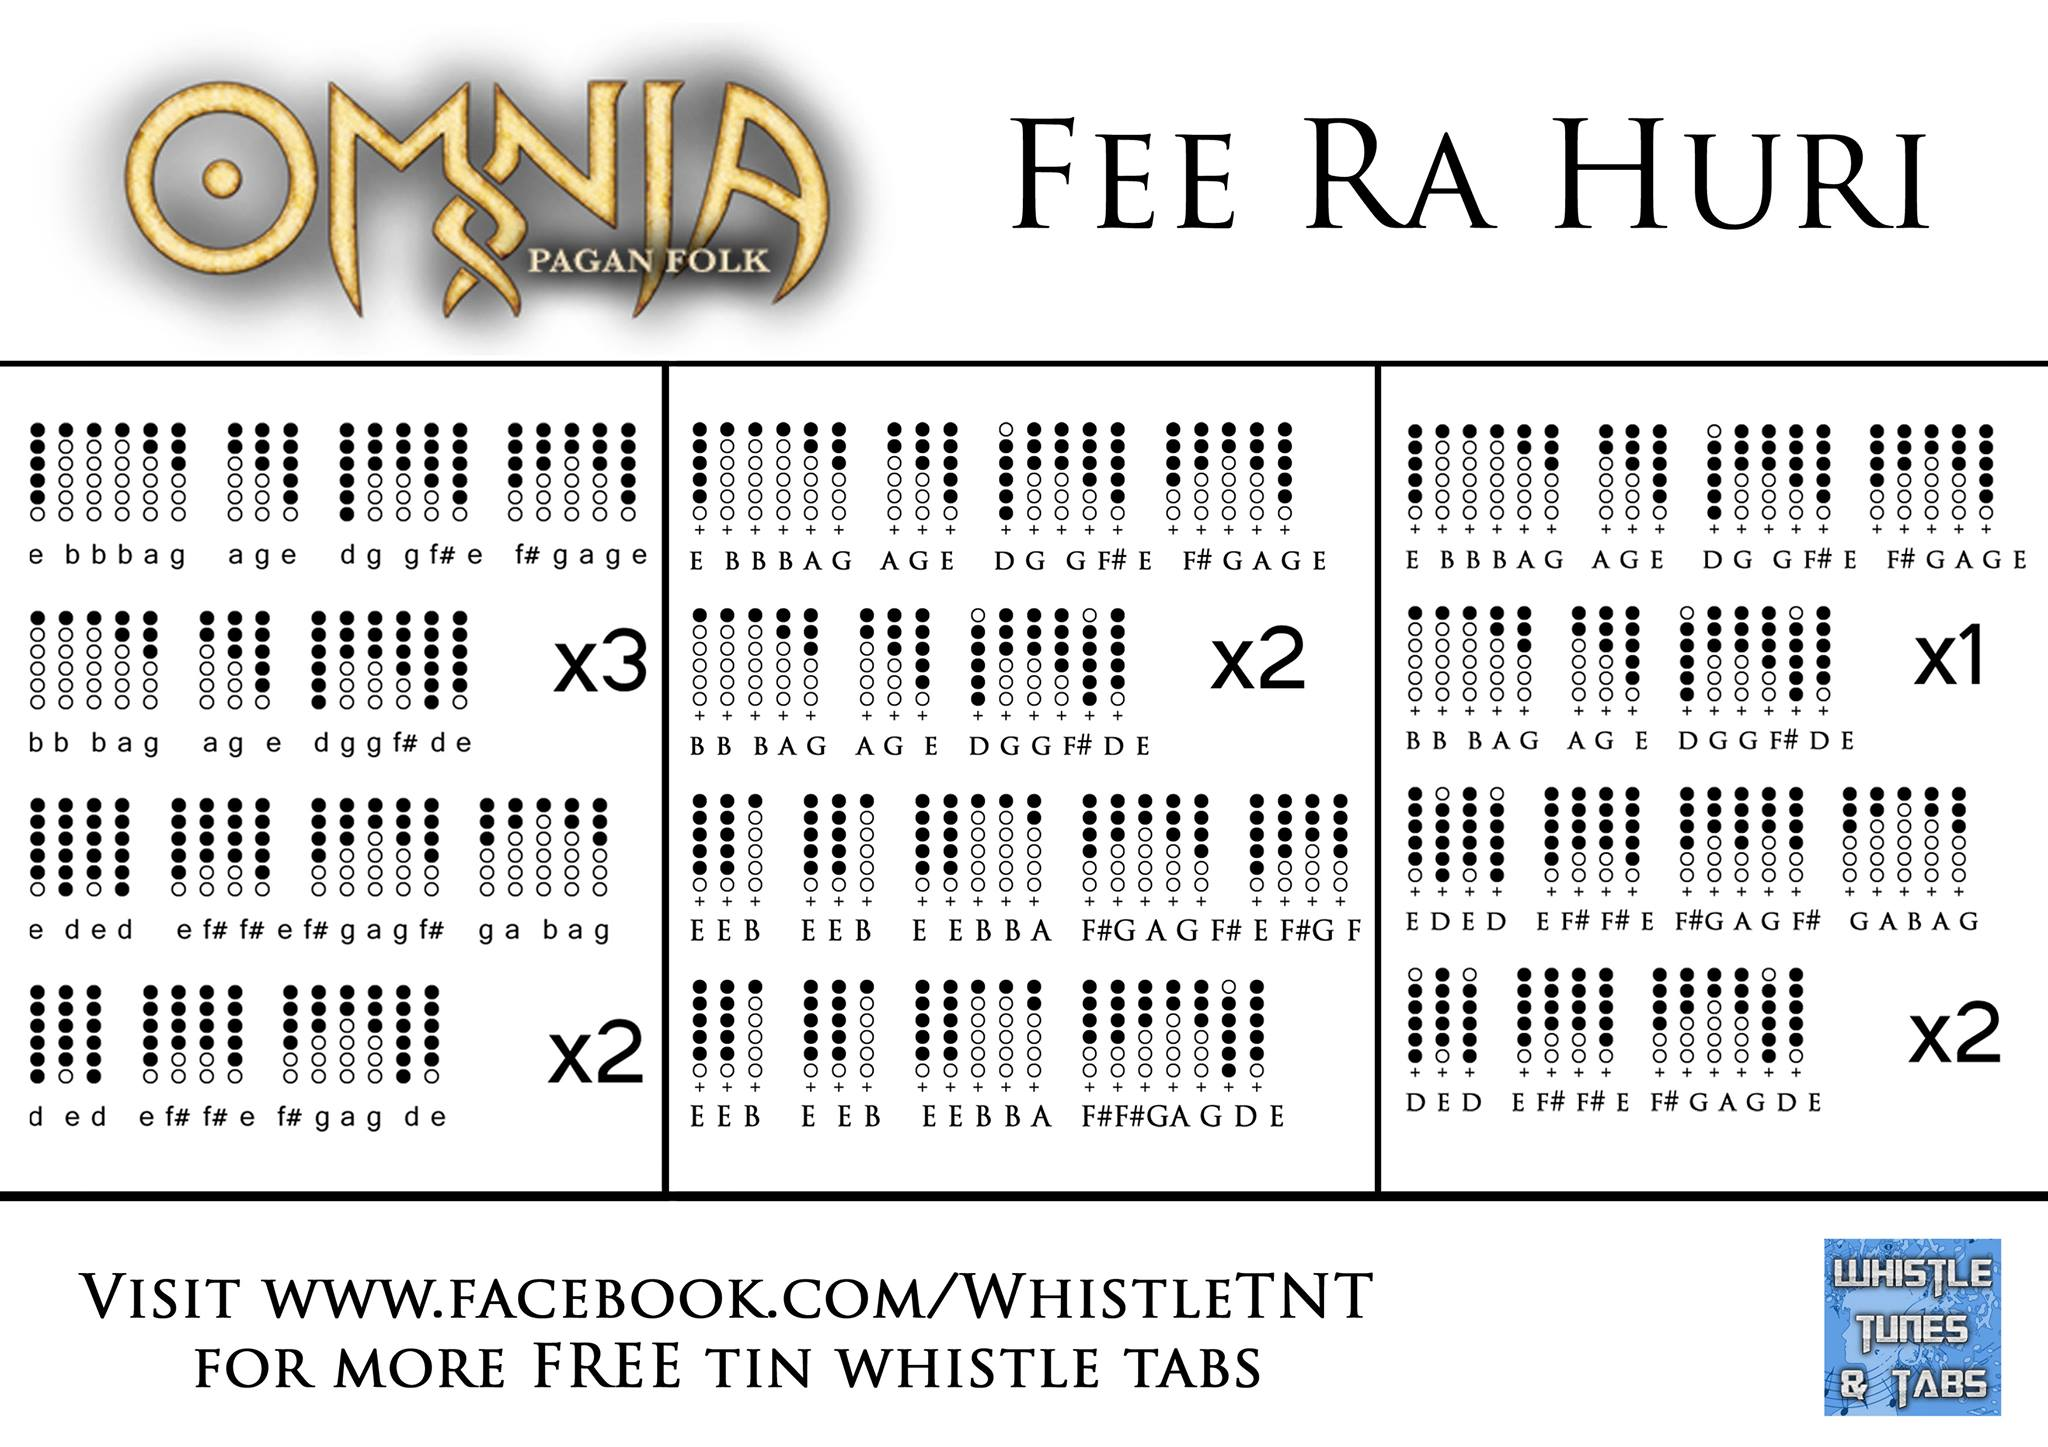
\includegraphics[width=0.8\textwidth]{./img/omnia.jpg}
% \caption[Popis do seznamu obrazku.]{Dlooooooouhy popis, co bude pod obrázkem.}
% \label{omnia.jpg}
% \end{figure}
% }

\chapter*{Závěr} % SEM NESAHEJTE!
\addcontentsline{toc}{chapter}{Závěr} % SEM NESAHEJTE!
\markboth{Závěr}{Závěr}
Zaver!!!


\printbibliography[heading=bibintoc]

\newpage
\appendix

\chapter*{Přílohy}
\addcontentsline{toc}{chapter}{Přílohy}
\renewcommand{\thesection}{\Alph{section}}

\section{Protokol z aproximace metriky pomocí HPELM}
\label{app:protocol}
\begin{figure}[H]
	\centering
	\includegraphics[scale=0.2]{img/largeprot100000-1-1.png}
\end{figure}
\begin{figure}[H]
	\centering
	\includegraphics[scale=0.25]{img/largeprot100000-2-1.png}
\end{figure}
\begin{figure}[H]
	\centering
	\includegraphics[scale=0.25]{img/largeprot100000-3-1.png}
\end{figure}
\begin{figure}[H]
	\centering
	\includegraphics[scale=0.25]{img/largeprot100000-4-1.png}
\end{figure}
\begin{figure}[H]
	\centering
	\includegraphics[scale=0.25]{img/largeprot100000-5-1.png}
\end{figure}
\begin{figure}[H]
	\centering
	\includegraphics[scale=0.25]{img/largeprot100000-6-1.png}
\end{figure}
\begin{figure}[H]
	\centering
	\includegraphics[scale=0.25]{img/largeprot100000-7-1.png}
\end{figure}
\begin{figure}[H]
	\centering
	\includegraphics[scale=0.25]{img/largeprot100000-8-1.png}
\end{figure}
\begin{figure}[H]
	\centering
	\includegraphics[scale=0.25]{img/largeprot100000-9-1.png}
\end{figure}
\begin{figure}[H]
	\centering
	\includegraphics[scale=0.25]{img/largeprot100000-10-1.png}
\end{figure}
\begin{figure}[H]
	\centering
	\includegraphics[scale=0.25]{img/largeprot100000-11-1.png}
\end{figure}
\begin{figure}[H]
	\centering
	\includegraphics[scale=0.25]{img/largeprot100000-12-1.png}
\end{figure}
\begin{figure}[H]
	\centering
	\includegraphics[scale=0.25]{img/largeprot100000-13-1.png}
\end{figure}
\begin{figure}[H]
	\centering
	\includegraphics[scale=0.25]{img/largeprot100000-14-1.png}
\end{figure}
\begin{figure}[H]
	\centering
	\includegraphics[scale=0.25]{img/largeprot100000-15-1.png}
\end{figure}
\begin{figure}[H]
	\centering
	\includegraphics[scale=0.25]{img/largeprot100000-16-1.png}
\end{figure}
% \includepdf[pages={2,3,4,5,6,7,8,9,10,11,12,13,14,15,16}]{img/largeprot100000.pdf}
\newpage
\section{Veličiny použité pro popis palivových souborů.}
\label{app:params}
\begin{table}[h]
\footnotesize
\centering
\caption{Veličiny pro popis palivových souborů.}
\label{tab:fap_gen}
%\resizebox{\textwidth}{!}{%
\begin{tabular}{|c|c|c|}
\hline
\tb{Veličina} & \tb{Jednotka} & \tb{Popis} \\ \hline
\verb|kinf| & -- & \makecell{Koeficient násobení nekonečného reaktoru \\ (z daného palivového souboru,\\ vypočteno kódem)} \\ \hline
\verb|kinf_lib| & -- & \makecell{Koeficient násobení nekonečného reaktoru \\ (z daného palivového souboru,\\ referenční hodnota z knihovny)} \\ \hline
\verb|rho_mod| & \jdt{kg\cdot m^{-3}} & Hustota moderátoru (\jdt{H_2 O}) \\ \hline
\verb|t_mod| & \jdt{\degree C} & Teplota moderátoru (\jdt{H_2 O}) \\ \hline
\verb|t_fuel| & \jdt{\degree C} & Teplota paliva \\ \hline
\verb|burnup| & \jdt{MWd\cdot (kg~U)^{-1}} & Vyhoření \\ \hline
\verb|power| & \jdt{W\cdot cm^{-1}} & Lineární hustota výkonu \\ \hline
\verb|c_h3bo3| & \jdt{g\cdot kg^{-1}} & Koncentrace \jdt{H_3 BO_3} \\ \hline
\verb|pnl| & s & Doba života okamžitých neutronů \\ \hline
\makecell{\texttt{rflux\_1} \\ \texttt{rflux\_2}} & -- & \makecell{Relativní hustota toku neutronů \\ v 1., resp. 2. grupě} \\ \hline
\makecell{\texttt{velocity\_1} \\ \texttt{velocity\_2}} & \jdt{m\cdot s^{-1}} & \makecell{Rychlost neutronů \\ v 1., resp. 2. grupě} \\ \hline
\makecell{\texttt{y\_i135} \\ \texttt{y\_xe135}} & -- & Výtěžek \ce{^{135}I}, resp. \ce{^{135}Xe} \\ \hline
\end{tabular}

\end{table}

\begin{table}[h]
\scriptsize
\centering
\caption{Účinné průřezy pro popis palivových souborů.}
\label{tab:fap_sigma}
\begin{tabular}{|c|c|c|c|c|c|c|c|}
\hline
\multicolumn{2}{|c|}{\tb{2G} $\bv{\Sigma_a}$} & \multicolumn{2}{c|}{\tb{2G} $\bv{\Sigma}$} & \tb{1G} $\bv{\Sigma}$ & \tb{2G} $\bv{\sigma_a}$ & \multicolumn{2}{c|}{\makecell{\tb{2G} $\bv{\sigma}$ \\ \tb{(neznačené jsou absorpční)}}} \\ \hline
\texttt{sa\_0\_1} & \texttt{sa\_0\_2} & \texttt{ss1\_1} & \texttt{ss2\_1} & \texttt{a\_xe135} & \texttt{msa\_gd152\_1} & \texttt{micro\_f\_u235\_1} & \texttt{micro\_f\_u235\_2} \\ \hline
\texttt{sa\_b\_1     }& \texttt{sa\_b\_2     }& \texttt{ss1\_2 }& \texttt{ss2\_2 }& \texttt{c\_u235  }& \texttt{msa\_gd155\_1 }& \texttt{micro\_f\_u238\_1  }& \texttt{micro\_f\_u238\_2 }\\ \hline
\texttt{sa\_gd\_1    }& \texttt{sa\_gd\_2    }& \texttt{nf1   }& \texttt{nf2    }& \texttt{a\_u236  }&  \texttt{msa\_gd156\_1 }& \texttt{micro\_f\_pu239\_1 }& \texttt{micro\_f\_pu239\_2} \\ \hline
\texttt{sa\_gd152\_1 }& \texttt{sa\_gd152\_2 }& \texttt{kf1   }& \texttt{kf2    }& \texttt{c\_u238  }& \texttt{msa\_gd157\_1 }& \texttt{micro\_c\_u235\_1  }& \texttt{micro\_c\_u235\_2} \\ \hline
\texttt{sa\_gd155\_1 }& \texttt{sa\_gd155\_2 }& \texttt{ds1   }& \texttt{ds2    }& \texttt{c\_pu239 }& \texttt{msa\_gd158\_1 }& \texttt{micro\_c\_u238\_1  }& \texttt{micro\_c\_u238\_2} \\ \hline
\texttt{sa\_gd156\_1 }& \texttt{sa\_gd156\_2 }& \texttt{df1   }& \texttt{df2    }& \texttt{a\_pu240 }& \texttt{msa\_gd160\_1 }& \texttt{micro\_c\_pu239\_1 }& \texttt{micro\_c\_pu239\_2} \\ \hline
\texttt{sa\_gd157\_1 }& \texttt{sa\_gd157\_2 }& \texttt{sf1   }& \texttt{sf2    }& \texttt{c\_pu241 }& \texttt{msa\_gd152\_2 }& \texttt{micro\_b10\_1     }& \texttt{micro\_b10\_2} \\ \hline
\texttt{sa\_gd158\_1 }& \texttt{sa\_gd158\_2 }& \texttt{d1    }& \texttt{d2     }& \texttt{f\_pu239 }& \texttt{msa\_gd155\_2 }& \texttt{micro\_xe135\_1   }& \texttt{micro\_xe135\_2} \\ \hline
\texttt{sa\_gd160\_1 }& \texttt{sa\_gd160\_2 }& \texttt{ch1   }& \texttt{ch2    }& \texttt{f\_pu241 }& \texttt{msa\_gd156\_2 }&  &  \\ \hline
\texttt{sa\_xe\_1    }& \texttt{sa\_xe\_2    }& \texttt{sa1   }& \texttt{sa2    }& \texttt{f\_u235  }& \texttt{msa\_gd157\_2 }&  &  \\ \hline
\texttt{sa\_sm\_1    }& \texttt{sa\_sm\_2    }&  &  & \texttt{f\_u238 }& \texttt{msa\_gd158\_2 }&  &  \\ \hline
		      &  &  &  &  & \texttt{msa\_gd160\_2} &  &  \\ \hline
\end{tabular}
\end{table}
\newpage
\section{Obsah přiloženého CD}
\begin{itemize}
\item Tato práce ve formátu PDF (bp\_rzehulka2020.pdf).
\item Použitá data před zpracováním -- složka data.
\item Skript codedatapreparationextractFuelParameters.rb, napsaný v jazyce Ruby, načítající soubor u1c15.fap.csv, vytvoří soubor fapSorted.csv, kde jsou \ac{ps} seřazeny k dalšímu použití.
\item Složka matlab se zdrojovými kódy v MATLABu k fitování.
	\cit{
	\item Soubor configSample.json k nastavení parametru modelu (metoda, množství dat, minimální velikost listu u regression tree ensamble,...).
	\item Funkci makeMod.m načítající parametry z config.json| souboru a volající funkci computeLocal a případně pomocnou funkci renameOutputs. 
	\item Pomocná funkce renameOutputs.m k unikátnímu pojmenování výstupních souborů.
	\item Funkce computeLocal.m načítající MATLAB Workspace s maicí konfigurací $C$, odezev $R$ a 3D maticí parametrů \ac{ps} FAP. Dále volá funkci 
		createTrainData2. Na vytvořená datech volá funkci k tvorbě modelu. Nakonec vše uloží.
	\item Funkce createTrainData2.m vybírající náhodnou podmnožinu $C$ a $R$ dané velikosti. Volá funkci createP a tvoří rozdíl norem \ac{ps} 
		v \ac{az}.
	\item Funkce createP.m vybírá z matice FAP parametry daného \ac{ps} v dané rotaci.
	\item Funkce trainModel.m tvořící model z vytvořených dvojic.


	}
\item Složka codehpelmpairs obsahující:
	\cit{
	\item Skript gpurunpairs.py, používaný k vytvoření párů vstupních dat, odečtení rozdílu jejich parametrů a nafitování metodou \ac{hpelm}. 
		Vytvořený model postupně otestuje, uloží grafy z testování a nakonec vytvoří zdrojový soubor tex k tvorbě protokolu.
	\item Skript myfunc.py obsahující pomocné funkce pro skript gpurunpairs.py.
	\item Soubor config.json určený k nastavení paraemetrů fitovaného modelu (množství dat, počet neuronů,...).
	}
\item Složka nfsolver obsahuje následující:
	\cit{
	\item Skript creator.ipynb, načítající konfigurace, odezvy a fapSorted.csv. Provádí normalizaci nebo standardizaci výstupů a tvorbu 
		vstupního datasetu, včetně odstranění konstantních hodnot a normalizace nebo standardizace a uložení do vhodného formátu (např. Apache Parquet).
	\item Skript pca.ipynb, používaného pro provedení PCA transformace vstupních dat.
	\item Skript hpelmnfsolverhpelmnfsolver.ipynb, používaný pro pokusy aproximovat neutronický kód metodou \ac{hpelm}.
	\item Skript tfnfsolvertffitnfsolver.ipynb, používaný pro pokusy aproximovat neutronický kód metodou \ac{dnn}.
	}
\end{itemize}


\end{document}
